\documentclass{ctexart}
\title{系统开发工具基础第二次实验报告}
\author{张烨 23020007162}
\date{\today}
\usepackage{graphicx}
\usepackage{float}
\graphicspath{{figures/}}
\ctexset{
	section={
		%format用于设置章节标题全局格式,作用域为标题和编号
		%字号为小三,字体为黑体,左对齐
		%+号表示在原有格式下附加格式命令
		format+ = \zihao{-3} \heiti \raggedright,
		%name用于设置章节编号前后的词语
		%前、后词语用英文状态下,分开
		%如果没有前或后词语可以不填
		name = {,、},
		%number用于设置章节编号数字输出格式
		%输出section编号为中文
		number = \chinese{section},
		%beforeskip用于设置章节标题前的垂直间距
		%ex为当前字号下字母x的高度
		%基础高度为1.0ex,可以伸展到1.2ex,也可以收缩到0.8ex
		beforeskip = 1.0ex plus 0.2ex minus .2ex,
		%afterskip用于设置章节标题后的垂直间距
		afterskip = 1.0ex plus 0.2ex minus .2ex,
		%aftername用于控制编号和标题之间的格式
		%\hspace用于增加水平间距
		aftername = \hspace{0pt}
	},
	subsection={
		format+ = \zihao{4} \kaishu \raggedright,
		%仅输出subsection编号且为中文
		number = \chinese{subsection},
		name = {(,)},
		beforeskip = 1.0ex plus 0.2ex minus .2ex,
		afterskip = 1.0ex plus 0.2ex minus .2ex,
		aftername = \hspace{0pt}
	},
	subsubsection={
		%设置对齐方式为居中对齐
		format+ = \zihao{-4} \fangsong \centering,
		%仅输出subsubsection编号,格式为阿拉伯数字,打字机字体
		number = \ttfamily\arabic{subsubsection},
		name = {,.},
		beforeskip = 1.0ex plus 0.2ex minus .2ex,
		afterskip = 1.0ex plus 0.2ex minus .2ex,
		aftername = \hspace{0pt}
	}
}

\begin{document}
	\maketitle
	\tableofcontents
	\newpage
	\section{实验目的}
	\section{实验内容}
	\subsection{Shell}
	\subsubsection{脚本格式和执行命令}
	脚本以\verb|#!/bin/bash|开头,下面是一个例子:
	
	\begin{figure}[H]
		\centering
		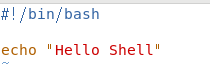
\includegraphics{2.1}
		\caption{shell脚本}
	\end{figure}
	
	shell脚本执行命令:\verb|./test.sh|或\verb|sh test.sh|,但是两者存在差异。
	
	\verb|./test.sh|:这种方式通过直接调用脚本文件来执行。要使用这种方式,脚本文件必须具有执行权限。使用chmod命令赋予脚本执行权限。
	
	\verb|sh test.sh|:这种方式通过指定的shell解释器来执行脚本。脚本文件不需要有执行权限,只要脚本文件可读即可。
	
	下面是一个例子:
	
	\begin{figure}[H]
		\centering
		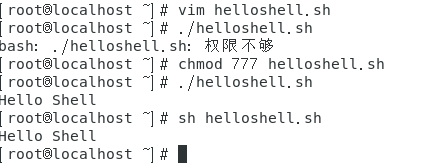
\includegraphics{2.2}
		\caption{脚本执行}
	\end{figure}
	
	\subsubsection{shell中的变量——自定义变量、静态变量、全局变量}
	变量定义规则:
	
	(1)变量名称可以由字母,数字和下划线组成,不能以数字开头,环境变量名建议大写
	
	(2)等号两侧不能有空格
	
	(3)在bash中,变量默认类型都是字符串类型,无法直接进行数值运算
	
	(4)变量的值如果有空格,需要使用双引号或单引号括起来
	
	
	
	1.自定义变量
	
	格式:变量=值 等号两边不能留有空格
	
	撤销变量:unset变量
	
	输出变量:echo \verb|$|变量
	
	\begin{figure}[H]
		\centering
		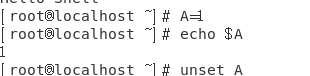
\includegraphics{2.3}
		\caption{变量}
	\end{figure}
	
	2.静态变量
	
	格式:readonly 变量
	
	注意:静态变量不能撤销
	
	\begin{figure}[H]
		\centering
		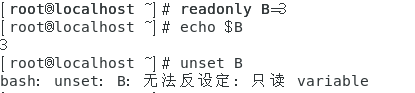
\includegraphics{2.4}
		\caption{静态变量}
	\end{figure}
	
	3.全局变量
	
	格式:export 变量
	
	全局变量可以在其他shell程序使用
	
	\begin{figure}[H]
		\centering
		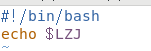
\includegraphics{2.6}
		\caption{全局变量}
	\end{figure}
	
	\begin{figure}[H]
		\centering
		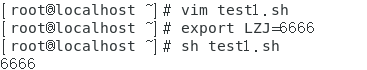
\includegraphics{2.7}
		\caption{全局变量}
	\end{figure}
	
	\subsubsection{特殊变量}
	
	1.\verb|$n|
	
	n为数字,\verb|$0|代表脚本名称,10以内参数用\verb|$1-9| 表 示 , 10 以 上 的 需 要 用 大 括 号 包 含
	
	\begin{figure}[H]
		\centering
		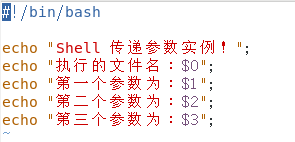
\includegraphics{2.11}
		\caption{1}
	\end{figure}
	
	\begin{figure}[H]
		\centering
		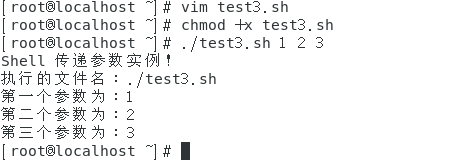
\includegraphics{2.10}
		\caption{1}
	\end{figure}
	
	2.\verb|$#|
	
	\verb|$#|:用于获取所有输入参数个数,常用于循环。
	
	\begin{figure}[H]
		\centering
		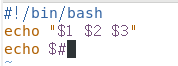
\includegraphics{2.12}
		\caption{2}
	\end{figure}
	
	\begin{figure}[H]
		\centering
		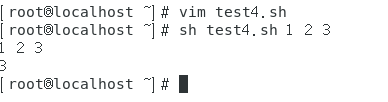
\includegraphics{2.13}
		\caption{2}
	\end{figure}
	
	3.\verb|$* $@ $?|
	
	\verb|$*|:代表命令行中所有的参数,把所有参数看成一个整体
	
	\verb|$@|:代表命令行中所有的参数,不过把每个参数区分对待
	
	\verb|$?|:最后一次执行状态命令的状态 0 表示正确执行
	
	\begin{figure}[H]
		\centering
		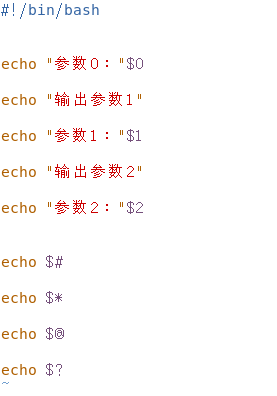
\includegraphics{2.14}
		\caption{3}
	\end{figure}
	
	\begin{figure}[H]
		\centering
		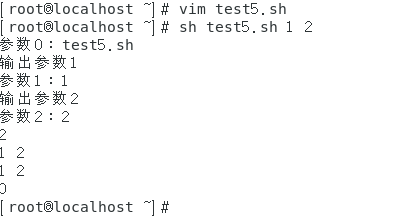
\includegraphics{2.15}
		\caption{3}
	\end{figure}
	
	\subsubsection{运算符}
	基本语法:
	
	1.expr \verb|+、-、*、/、%| 运算符之间要有空格
	
	2.\verb|$|((运算式))或\verb|$|[运算式]
	
	\begin{figure}[H]
		\centering
		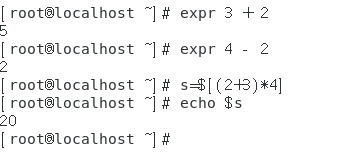
\includegraphics{2.16}
		\caption{运算符}
	\end{figure}
	
	\subsubsection{条件判断}
	
	两个整数之间比较:
	
	\begin{table}[h]
		\centering
		\caption{整数}
		\begin{tabular}{|c|c|}
			\hline
			符号 & 描述  \\
			\hline
			-lt & 小于 \\
			\hline
			-le & 小于等于\\
			\hline
			-eq &等于\\ 
			\hline
			-gt & 大于\\
			\hline
			-ge & 大于等于\\
			\hline
			-ne & 不等\\
			\hline
		\end{tabular}
	\end{table}
	
	文件权限判断:
	
	\begin{table}[h]
		\centering
		\caption{文件}
		\begin{tabular}{|c|c|}
			\hline
			符号 & 描述  \\
			\hline
			-r & 有读的权限 \\
			\hline
			-w & 有写的权限\\
			\hline
			-x &有执行的权限\\ 
			\hline
		\end{tabular}
	\end{table}
	
	文件类型判断:
	
	\begin{table}[h]
		\centering
		\caption{文件类型}
		\begin{tabular}{|c|c|}
			\hline
			符号 & 描述  \\
			\hline
			-f & 文件存在并且是一个常规文件 \\
			\hline
			-e & 文件存在\\
			\hline
			-d &文件存在并且是一个目录\\ 
			\hline
		\end{tabular}
	\end{table}
	
	
	\begin{figure}[H]
		\centering
		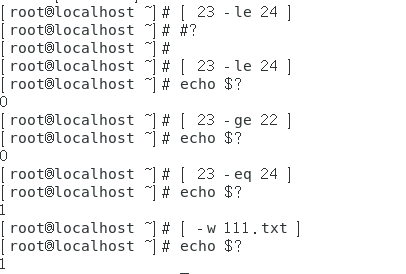
\includegraphics{2.17}
		\caption{比较}
	\end{figure}
	
	多条件判断:
	
	\verb|&&|表示前一条命令执行成功时,才执行后一条命令
	
	\verb||||表示上一条命令执行失败后,才执行下一条命令
	
	\begin{figure}[H]
		\centering
		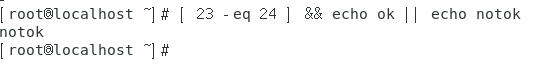
\includegraphics{2.18}
		\caption{多条件判断}
	\end{figure}
	
	\subsubsection{if判断}
	1.基本语法
	
	if [ 条件判断式 ];then
	
	\quad \quad 程序
	
	fi
	
	或者
	
	if [ 条件判断式 ]
	
	then
	
	\quad \quad 程序
	
	fi
	
	多条件判断
	
	if [ 条件判断式 ]
	
	then
	
	\quad \quad 程序
	
	elif [ 条件判断式 ]  
	
	then 
	
	\quad \quad 程序
	
	fi
	
	2.注意事项:
	
	(1)中括号和条件判断式之间必须有空格
	
	(2)if后要有空格
	
	下面是一个例子:
	
	\begin{figure}[H]
		\centering
		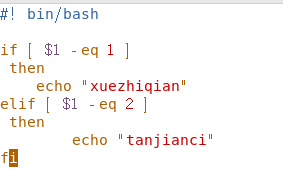
\includegraphics{2.19}
		\caption{if判断}
	\end{figure}
	
	\begin{figure}[H]
		\centering
		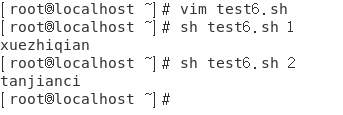
\includegraphics{2.20}
		\caption{if判断}
	\end{figure}
	
	\subsubsection{case语句}
	
	1.基本语法
	
	case \verb|$|变量名 in
	
	"值1")
	
	   \quad \quad 程序1
	
	   \quad \quad ;;
	
	"值2")
	
	   \quad \quad 程序2
	
	   \quad \quad ;;
	
	*)
	
	   \quad \quad 变量都不是以上值,则执行此程序
	
	   \quad \quad ;;
	
	esac
	
	2.注意事项
	
	(1)case行尾必须为单词“in”,每个模式匹配必须以“)”结束
	
	(2)双分号“;;”表示命令序列结束,相当于break
	
	(3)最后的“*)”表示默认模式,相当于default
	
	下面是一个例子:
	
	\begin{figure}[H]
		\centering
		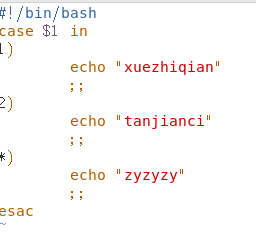
\includegraphics{2.21}
		\caption{case语句}
	\end{figure}
	
	\begin{figure}[H]
		\centering
		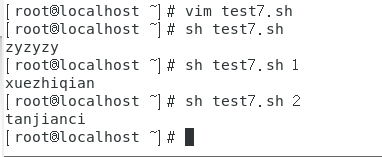
\includegraphics{2.22}
		\caption{case语句}
	\end{figure}
	
	\subsubsection{for循环}
	
	基本语法
	
	for((初始值;循环控制;条件变量变化))
	
	do
	
	\quad \quad 程序
	
	done
	
	或
	
	for 变量 in 值1 值2 值3
	
	do
	
	\quad \quad 程序
	
	done 
	
	下面是一个例子:
	
	\begin{figure}[H]
		\centering
		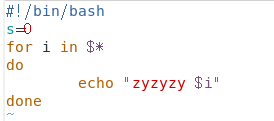
\includegraphics{2.23}
		\caption{for循环}
	\end{figure}
	
	\begin{figure}[H]
		\centering
		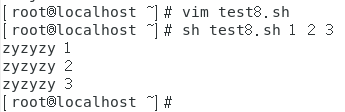
\includegraphics{2.24}
		\caption{for循环}
	\end{figure}
	
	\subsubsection{while循环}
	
	基本语法
	
	while [ 条件判断式 ]
	
	do
	
	\quad \quad 程序
	
	done 
	
	下面是一个例子:
	
	\begin{figure}[H]
		\centering
		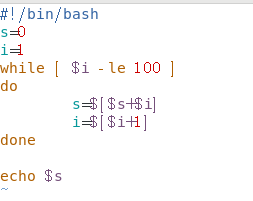
\includegraphics{2.25}
		\caption{while循环}
	\end{figure}
	
	\begin{figure}[H]
		\centering
		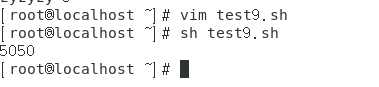
\includegraphics{2.26}
		\caption{while循环}
	\end{figure}
	
	\subsubsection{函数}
	
	基本语法
	
	[function] funname[()]
	
	{
		
		\quad \quad Action;
		
		\quad \quad [return int;]
		
	}
	
	funname
	
	下面是一个例子:
	
	\begin{figure}[H]
		\centering
		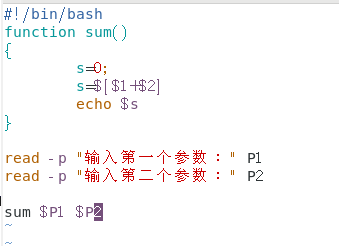
\includegraphics{2.27}
		\caption{函数}
	\end{figure}
	
	\begin{figure}[H]
		\centering
		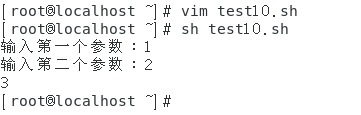
\includegraphics{2.28}
		\caption{函数}
	\end{figure}
	
	\subsubsection{不同的ls命令}
	
	\begin{figure}[H]
		\centering
		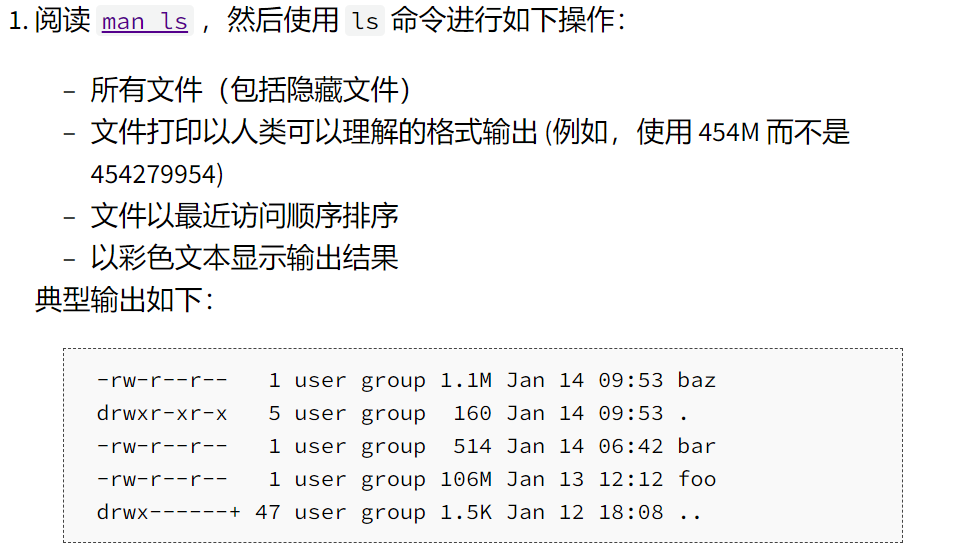
\includegraphics{2.29}
		\caption{问题}
	\end{figure}
	
	\begin{figure}[H]
		\centering
		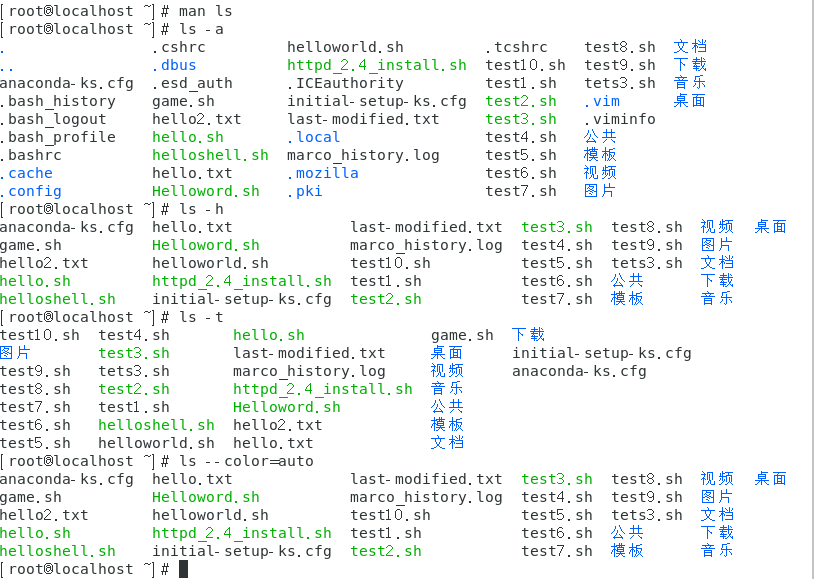
\includegraphics{2.30}
		\caption{解答}
	\end{figure}
	
	\subsubsection{编写marco和polo函数}
	
	\begin{figure}[H]
		\centering
		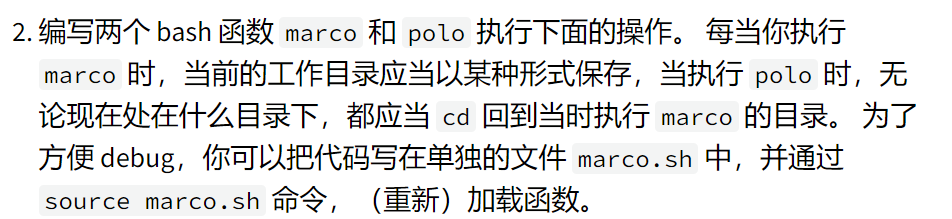
\includegraphics{2.31}
		\caption{问题}
	\end{figure}
	
	\begin{figure}[H]
		\centering
		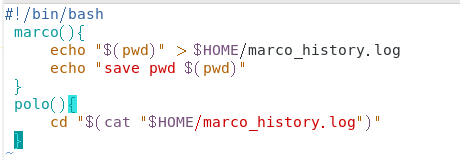
\includegraphics{2.32}
		\caption{函数}
	\end{figure}
	
	\begin{figure}[H]
		\centering
		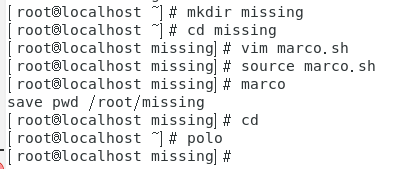
\includegraphics{2.33}
		\caption{执行}
	\end{figure}
	
	为了让结果更清晰,新建了missing目录,可以看到,当执行polo函数时,回到了当时执行marco的目录。
	
	
	\subsection{Vim}
	\subsubsection{三种模式}
	1.命令模式:不能对文件直接编辑,只能通过快捷键进行一些操作(如移动光标、复制、粘贴等),打开vim后默认进入命令模式
	
	2.末行模式:可在末行输入一些命令对文件进行操作(如搜索、替换、保存、退出、高亮等)
	
	3.编辑模式:可对文件内容进行编辑
	\subsubsection{vim的进入和退出}
	
	1.进入
	
	(1)vim 文件路径 :直接打开指定文件
	
	(2)vim +数字 文件路径 :打开指定文件并将光标移动到指定行
	
	\begin{figure}[H]
		\centering
		
\includegraphics{2.35}
		\caption{指定第四行}
	\end{figure}
	
	\begin{figure}[H]
		\centering
		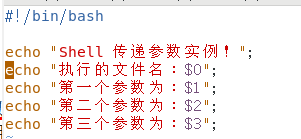
\includegraphics{2.34}
		\caption{查看}
	\end{figure}
	
	可以看到,打开文件后光标在第四行
	
	
	(3)vim +/关键词 文件路径 :打开指定文件并高亮显示关键词
	
	\begin{figure}[H]
		\centering
		
\includegraphics{2.37}
		\caption{关键词echo}
	\end{figure}
	
	\begin{figure}[H]
		\centering
		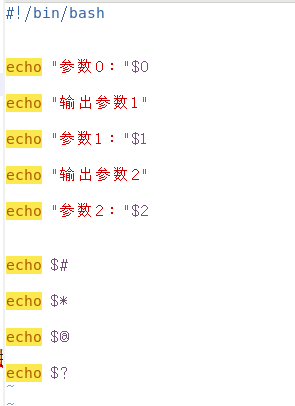
\includegraphics{2.36}
		\caption{查看}
	\end{figure}
	
	设置关键词为echo,可以看到,打开文件后echo被高亮显示
	
	(4)vim 文件路径1 文件路径2 文件路径3 :同时打开多个文件,文件之间可切换操作
	
	\subsubsection{移动光标}
	虽然可以直接使用↑ ↓ ← → 进行移动,但正规的是:
	
	\begin{table}[h]
		\centering
		\caption{移动光标}
		\begin{tabular}{|c|c|}
			\hline
			符号 & 描述  \\
			\hline
			h & 左 \\
			\hline
			j & 下\\
			\hline
			k &上\\ 
			\hline
			l & 右\\
			\hline
		\end{tabular}
	\end{table}

	
	\subsubsection{简单计算器}
	在编辑模式下ctrl+r,然后点击=,光标就会移动到末行,输入要计算的式子,按下enter,计算结果就会出现在原光标位置处
	
	\begin{figure}[H]
		\centering
		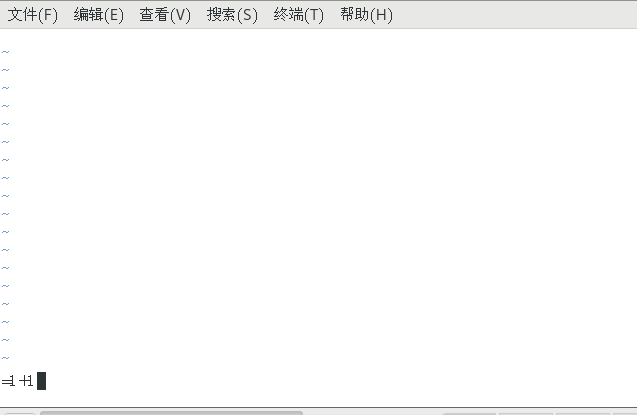
\includegraphics[scale=0.5]{2.38}
		\caption{计算器}
	\end{figure}
	
	\begin{figure}[H]
		\centering
		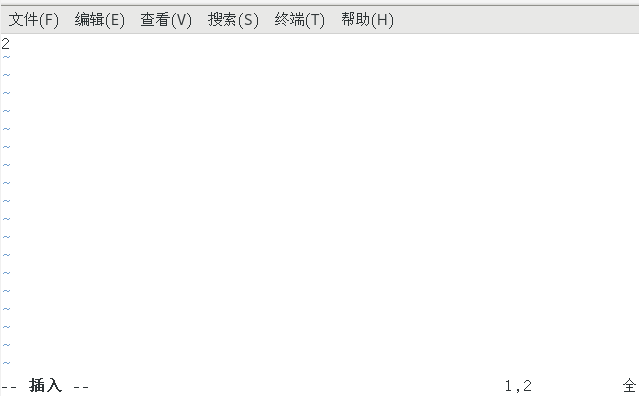
\includegraphics[scale=0.5]{2.39}
		\caption{计算器}
	\end{figure}
	
	\subsubsection{查找}
	当我们想要查找指定字符时,可以切换到底行模式下,输入?和字符,下面是一个查找hello的例子:
	
	\begin{figure}[H]
		\centering
		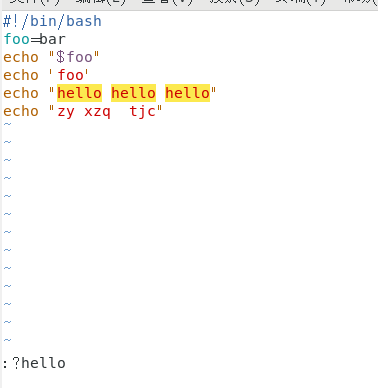
\includegraphics[scale=0.5]{2.40}
		\caption{hello}
	\end{figure}
	
	可以看到,在底行模式下输入:?hello,按下enter键后hello就会被高亮显示。
	
	\subsubsection{替换}
	切换到底行模式下,输入\verb|%s/string1/string2/g|,把string1替换成string2,下面把hh替换为hello
	\begin{figure}[H]
		\centering
		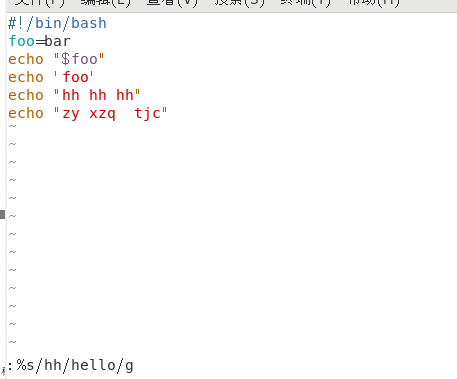
\includegraphics[scale=0.5]{2.41}
		\caption{hh}
	\end{figure}
	\begin{figure}[H]
		\centering
		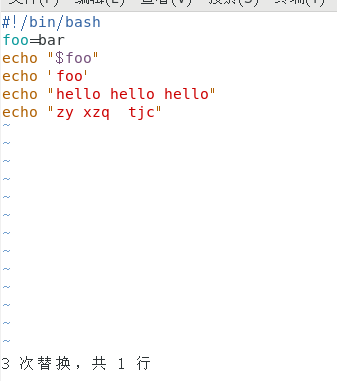
\includegraphics[scale=0.5]{2.42}
		\caption{hello}
	\end{figure}
	
	可以看到,hh被换成了hello
	
	\subsubsection{保存及退出}
	下面是不同的指令对应的不同功能:
	
	\begin{table}[h]
		\centering
		\caption{移动光标}
		\begin{tabular}{|c|c|}
			\hline
			符号 & 描述  \\
			\hline
			q & 直接退出\\
			\hline
			q! & 强制退出\\
			\hline
			w &保存\\ 
			\hline
			wq & 保存并退出\\
			\hline
			wq!&保存并强制退出\\
			\hline
		\end{tabular}
	\end{table}
	
	\subsubsection{调用外部命令}
	切换到底行模式下,输入:!和外部命令,比如说外部命令ls,就是:!ls
	\begin{figure}[H]
		\centering
		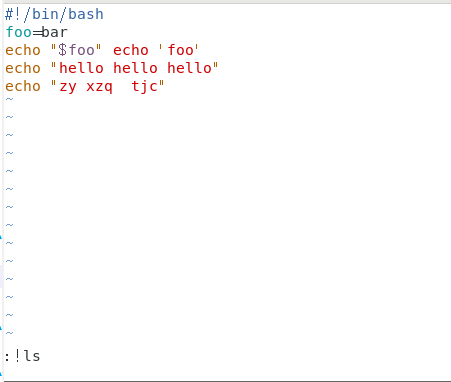
\includegraphics{2.44}
		\caption{ls}
	\end{figure}
	
	enter回车后就可以看到:
	\begin{figure}[H]
		\centering
		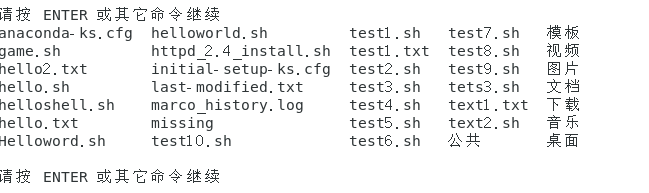
\includegraphics{2.45}
		\caption{ls}
	\end{figure}

	\section{心得体会}
	通过学习,掌握了shell和vim的基础功能,同时对数据整理也有了一定的了解。这次学习丰富了自身技能,并激发了我的学习热情。
	\section{相关练习、报告和代码查看链接}
	本次报告相关练习、报告和代码均可以在https://kkgithub.com/zhangtantan77/work查看
\end{document}
